\documentclass{beamer}
\usetheme{metropolis} % Use metropolis theme

\usepackage[a-2u]{pdfx}
\usepackage[czech]{babel}
\usepackage[utf8]{inputenc}
\usepackage[T1]{fontenc}
\usepackage{lmodern}
\usepackage{textcomp}
\usepackage{sansmath}  % enables switching to serif fonts also in math env
\usepackage{chemformula}
\usepackage{chemfig}
\usepackage[
	font=tiny,
	labelfont={tiny}
]{caption}
\usepackage{tabularx}  % tables with fixed width
\usepackage{booktabs}  % better looking tables, more space after horizontal
% rule (use \midrule) and possibility of bold line usage (\toprule and
% \bottomrule)

%%% tikz
\usepackage{tikz}  % nice images in LaTeX
\usetikzlibrary{%
	arrows.meta,%
	shapes,%
	intersections,%
	decorations.markings,%  arrows
	decorations.pathmorphing,%  zigzag, snake and other paths
	calc,%
	positioning%  left = 1cm and 3cm of SomeNode
}

% TikZ macros
\newcommand{\mypgfextractangle}[3]{%
	\pgfmathanglebetweenpoints{%
		\pgfpointanchor{#2}{center}}{%
		\pgfpointanchor{#3}{center}}
	\global\let#1\pgfmathresult
}

\newcommand{\icm}{cm$^{-1}$}  % reciprocal centimeters
%%% upgright greek letters
\newcommand{\g}[1]{\foreignlanguage{greek}{#1}}


\title{Studium struktury a interakcí nukleových kyselin pomocí rezonančního
Ramanova rozptylu}
\date{}
%\date{15. prosince 2021}
%\author{Mgr. Jakub Klener}
%\institute{%
	%\parbox[c]{0.14\textwidth}{%
		%
\includegraphics[width=0.12\textwidth]{assets/logo.pdf}%
	%}%
	%\parbox[c]{0.8\textwidth}{Matematicko-fyzikální\\fakulta\\Univerzita Karlova}
%}
\author{%
	\parbox[c]{0.25\textwidth}{%
		
\includegraphics[width=0.22\textwidth]{assets/logo.pdf}%
	}%
	\parbox[c]{0.7\textwidth}{%
		Jakub Klener\\%
		Matematicko-fyzikální fakulta\\%
		Univerzita Karlova\\%
		15. prosince 2021
	}%
}

\begin{document}

\maketitle

\begin{frame}{Obsah}
  \setbeamertemplate{section in toc}[sections numbered]
  \tableofcontents[hideallsubsections]
\end{frame}


\section{Rezonanční Ramanův rozptyl a nukleové kyseliny}

\begin{frame}{Nukleové kyseliny}
\begin{itemize}
	\item Je tvořena kyselinou fosforečnou, pentózou a nukleovými bázemi
	\item Zabezpečují uchování a účastní se exprese genetické informace
	\item Mohou zaujmout mnoho různých konformací
\end{itemize}

\begin{figure}
	\centering
	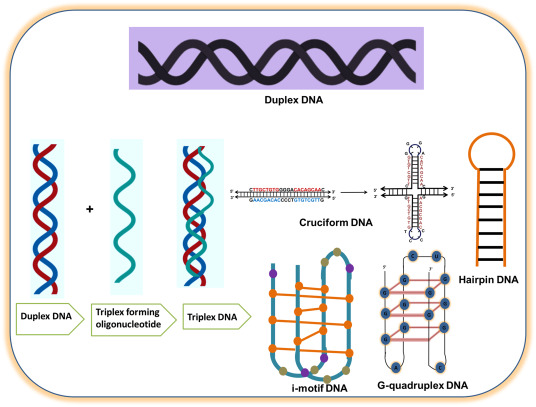
\includegraphics[width=.6\columnwidth]{assets/dna_conformations}
	\caption*{
		Pandia N. et al., 2021.
		\emph{Biochim. Biophis. Acta.}
		\textbf{1876}(2), 188594.
	}
\end{figure}
\end{frame}

\begin{frame}{Ramanova spektroskopie}
\begin{center}
	\resizebox{1\linewidth}{!}{\begin{tikzpicture}[line width=2, scale=1]
	\draw (0,0) -- ++(10.2,0);
	\draw (0,.6) -- ++(10.2,0);
	\draw (0,1.2) -- ++(10.2,0);
	\foreach \x in {0,.4, ...,10}
	{
		\draw [gray] (\x,4.5) -- ++(.2,0);
	}
	\draw (0,6) -- ++(10.2,0);
	\draw (0,6.6) -- ++(10.2,0);
	\draw (0,7.2) -- ++(10.2,0);

	\draw [->] (.5,0) -- ++(0,4.5);
	\draw [->] (1.5,4.5) -- ++(0,-4.5);

	\draw [->] (3.5,0) -- ++(0,4.5);
	\draw [->, color=red] (4.5,4.5) -- ++(0,-3.9);

	\draw [->] (6.5,0) -- ++(0,6.6);
	\draw [->, color=red] (7.5,6.6) -- ++(0,-6);

	\draw(1,0) node [below] {Rayleigh};
	\draw(4,0) node [below] {\textcolor{red}{Raman}};
	\draw(7,0) node [below] {\textcolor{red}{Rezonanční Raman}};
	\draw(0,4.5) node [left, align=right] {Virtuální\\hladiny};
	\draw(0,0.6) node [left, align=right] {Základní\\elektronový\\stav};
	\draw(0,6.6) node [left, align=right] {Excitovaný\\elektronový\\stav};

\end{tikzpicture}
}
\end{center}
\end{frame}

\begin{frame}{Proč UV rezonanční Ramanova spektroskopie?}
\begin{itemize}
	\item Zesílení, typicky o 1 -- 2 řády
	\item Zjednodušení spektra díky selektivnímu zesílení
	\item Hlavní třídy biomolekul mají elektronový absorpční přechod v~UV
	\item Fluorescence hlavně nečistot je i díky rezonančnímu přenosu často na
		větších vlnových délkách
\end{itemize}
\end{frame}


\section{Stavba spektrometru}

\begin{frame}{Design spektrometru}
\begin{center}
	\resizebox{1\linewidth}{!}{\begin{tikzpicture}[font=\Large\sffamily]

% settings
\newcommand*{\cellBorderWidth}{3\pgflinewidth}
\newcommand*{\cellLineWidth}{1.5\pgflinewidth}
\definecolor{glassBorderColor}{RGB}{0,128,255}
\definecolor{glassFillColor}{RGB}{230,242,255}
\definecolor{waterFillColor}{RGB}{0,128,255}
\definecolor{hclColor}{RGB}{255,128,0}
\definecolor{unwantedLightColor}{RGB}{153,17,0}
\tikzset{
	clip
}
\tikzset{
	mirror element/.style = {color = black, line width = 2 * \pgflinewidth},
	real laser beam/.style = {color = cyan, line width = 2 * \pgflinewidth},
	laser beam/.style = {real laser beam},
	scattered ray/.style = {color = red!60, line width = 1.5 * \pgflinewidth},
	scattered fill/.style = {fill = red, draw = none, fill opacity = 0.2},
	glass/.style = {color = glassBorderColor, opacity = 0.5,%
		fill = glassFillColor, fill opacity = 0.5},
	sample cell/.style = {color = glassBorderColor, opacity = 0.5,%
		double = glassFillColor, double distance = \cellBorderWidth,
		line width = \cellLineWidth, line cap = rect},
	water fill/.style = {fill = waterFillColor, fill opacity = 0.1},
	mirror surface/.style = {color = black!20, fill = black!10},
	nd filter/.style = {color = black, opacity = 0.2, fill = black,%
		fill opacity = 0.1},
	nd carousel/.style = {color = black, opacity = 0.4, fill = black,%
		fill opacity = 0.2},
	notch/.style = {color = black, opacity = 0.4, fill = black,%
		fill opacity = 0.1},
	aperture/.style = {color = black, line width = 2 * \pgflinewidth},
	aperture filldraw/.style = {color = black!40, fill = black!20,%
		clip even odd rule},
	clip even odd rule/.code = {\pgfseteorule},
	shutter/.style = {nd carousel},
	shutter blade/.style = {dashed, line width = 1.5 * \pgflinewidth,%
		opacity = 0.4},
	hcl/.style = {nd carousel},
	hcl lamp/.style = {color = black!40, line width = 3 * \pgflinewidth,%
		line cap = round},
	hcl ray/.style = {color = black, opacity = 0.2,%
		line width = 1.5 * \pgflinewidth},
	hcl beam/.style = {draw = none, fill = black, opacity = 0.1},
	beam blocker/.style = {mirror element},
	unwanted ray/.style = {color = unwantedLightColor,%
		line width = 1.5 * \pgflinewidth}
};
\clip (-.1,-2.1) rectangle (14,6.6);
\coordinate (shutter) at (11,6);
\newcommand*{\samplePosWidth}{10.9}
\newcommand*{\samplePosHeight}{3}
\newcommand*{\laserUpWidth}{10}
\coordinate (M1) at (13,6);
\coordinate (M2) at (13,\samplePosHeight);
\coordinate (BeamBlocker) at ($ (M2) + (-0.35,1.2) $);
\newcommand*{\beamBlockerWidth}{0.5}
\coordinate (samplePos) at (\samplePosWidth,\samplePosHeight);
\coordinate (laserUp) at (\laserUpWidth,\samplePosHeight);
\newcommand*{\cellWidth}{1};
\coordinate (cassegrainM1Center) at (\samplePosWidth - 0.5,\samplePosHeight);
\newcommand*{\cassegrainMARadius}{1.5}
\coordinate (cassegrainM2Center) at (\samplePosWidth - 0.7,\samplePosHeight);
\newcommand*{\cassegrainMBRadius}{0.4}
\newcommand*{\sqrttwo}{1.414213}
\coordinate (HCL) at (6,0);
\coordinate (AC1) at (6,1.2);  % calibration aperture
\coordinate (LC1) at (6,0.6);  % calibration lens
\coordinate (MS1Edge1) at (4.5,\samplePosHeight + 0.5);
\coordinate (MS1Edge2) at (3.5,\samplePosHeight - 0.5);
\coordinate (MC1Edge1) at (5.5,2.5);
\coordinate (MC1Edge2) at (6.5,1.5);
\coordinate (MC1Edge3) at (5.5,1.5);
\coordinate (MC2FlippedEdge1) at (4.4,2.5);
\newcommand*{\MCBFlippedH}{1.0};  % MC2 height
\newcommand*{\MCBFlippedD}{1.0};  % MC2 depth
\coordinate (parabolaFocus) at (3,0.4);
\coordinate (MS2Edge1) at (4.5,1);
\coordinate (MS2EdgeControl1) at (245:0.5);
\coordinate (MS2Edge2) at (3.5,0);
\coordinate (MS2EdgeControl2) at (17:0.3);
\newcommand*{\apertureOuterRadius}{0.3}
\newcommand*{\apertureInnerRadius}{0.1}
\newcommand*{\pbrot}{305}  % Pellin broca prism rotation

% Pellin-Broca prism path def
% B -----
% |      ----C
% |           \
% |            \
% A ----------- D
\coordinate (PBB) at ($ (M1) + (0.06,0.2) $);
\coordinate (PBA) at ($ (PBB) + (270 + \pbrot:0.6) $);
\coordinate (PBD) at ($ (PBA) + (0 + \pbrot:0.9) $);
\path[name path=PBBtoC] (PBB) -- ++(345 + \pbrot:10);
\path[name path=PBDtoC] (PBD) -- ++(120 + \pbrot:10);
\path[name intersections={of=PBBtoC and PBDtoC, by=PBC}];
\path[name path=PBAB] (PBA) -- (PBB);
\path[name path=PBBC] (PBB) -- (PBC);
\path[name path=PBDA] (PBD) -- (PBA);

% laser
\draw (0,5.5) rectangle ++(3,1) node[pos=.5] {laser};

% laser beam Pellin-Broca coordinates
\path[name path=LToPBAB] (shutter) -- (M1);
\path[name intersections = {of = LToPBAB and PBAB, by = PBAB1}];
\draw[real laser beam] (3,6) -- (shutter);
\path[name path=LToPBBC] (PBAB1) -- ++(340:2);
\path[name intersections = {of = LToPBBC and PBBC, by = PBBC1}];
\path[name path=LToPBDA] (M2) -- (M1);
\path[name intersections = {of = LToPBDA and PBDA, by = PBDA1}];

% Unvanted laser beam
\path[name path=ULToPBBC] (PBAB1) -- ++(347:2);
\path[name intersections = {of = ULToPBBC and PBBC, by = UPBBC1}];
\path[name path=ULToPBDA] (M2) -- ($ (M1) + (-0.12,0) $);
\path[name intersections = {of = ULToPBDA and PBDA, by = UPBDA1}];

% Draw unwanted beam
\draw[unwanted ray] (PBAB1) -- (UPBBC1) -- (UPBDA1)
	-- ($ (BeamBlocker) + (0.08,0) $);

% Draw laser beam
\draw[laser beam] (shutter) -- (PBAB1) -- (PBBC1) -- (PBDA1) -- (M2)
	-- (laserUp);

% neutral density filters
\newcommand*{\ndfilterA}{(3.5,5.8) rectangle ++(0.2,0.4)}
\newcommand*{\ndfilterB}{(3.5,5) rectangle ++(0.2,0.4)}
\draw[nd filter] \ndfilterA;
\draw[nd filter] \ndfilterB;
\draw[nd carousel] (3.45,4.9) rectangle ++(0.3,0.1);
\draw[nd carousel] (3.45,5.4) rectangle ++(0.3,0.4);
\draw[nd carousel] (3.45,6.2) rectangle ++(0.3,0.1);
\node[below] at (3.6,4.9) {Neutral density filters};

\draw[shutter blade] ($ (shutter) + (0,0.3) $) -- ++(0,-0.6);
\draw[shutter] ($ (shutter) + (-0.1,-0.3) $) -- ++(0.2,0) -- ++(0,-0.4)
	-- ++(-0.2,0) -- cycle;
\node[below] at ($ (shutter) + (0,-0.7) $) {shutter};

% Pellin-Broca prism
\draw[glass] (PBA) -- (PBB) -- (PBC) -- (PBD) -- cycle;
\node[above, shift = {(-0.5cm,-0.05cm)}] at (PBB) {Pellin-Broca};
% Mirror 2
\draw[glass] ($ (M2) + (0.2,0.2) $)
	-- node[below, shift = {(0.35cm,0.05cm)}, color = black, opacity = 1.0]{M2}
	($ (M2) + (-0.2,-0.2) $) -- ++(0,0.4) -- cycle;
% Mirror 3 - it should be under the beam so we have to draw it first
%\draw[glass] ($ (samplePos) + (-0.2,0.2) $) rectangle ++(0.4,-0.4);
%\node[above] at ($ (samplePos) + (0,0.5) $) {M3};


% Unwanted frequencies beam blocker
\draw[beam blocker] ($ (BeamBlocker) + (0.5 * \beamBlockerWidth,0) $)
	-- ++(-\beamBlockerWidth,0) node[left, shift = {(0.3cm, 0.3cm)}] {Beam blocker};

% Aperture 1
\draw[aperture] ($ (M2) + (-0.5,\apertureOuterRadius) $)
	node[above]{A1}
	-- ++(0,-\apertureOuterRadius + \apertureInnerRadius);
\draw[aperture] ($ (M2) + (-0.5,-\apertureOuterRadius) $)
	-- ++(0,\apertureOuterRadius - \apertureInnerRadius);
% aperture 2
\draw[aperture filldraw]
	(laserUp) circle (\apertureOuterRadius)
	(laserUp) circle (\apertureInnerRadius);

% Draw laser beam on top
\draw[laser beam] (laserUp) -- (samplePos);

% mirror M4
\draw[glass] ($ (laserUp) + (0.15,0.15) $) rectangle ++(-0.3,-0.3);

% Draw laser focusing lens
\newcommand*{\LARadius}{0.7}
\coordinate (L1Center) at (\laserUpWidth+1.6-\LARadius,\samplePosHeight);
\path[name path=L1Arc, shift={(L1Center)}]
	(270:\LARadius) arc (-90:90:\LARadius);
\path[name path=toL1Arc1] ($ (laserUp)  + (0,0.4) $) -- ++(10,0);
\path[name path=toL1Arc2] ($ (laserUp)  + (0,-0.4) $) -- ++(10,0);
\path[name intersections={of=L1Arc and toL1Arc1, by=L11}];
\mypgfextractangle{\LAAAngle}{L1Center}{L11}
\path[name intersections={of=L1Arc and toL1Arc2, by=L12}];
\mypgfextractangle{\LABAngle}{L1Center}{L12}
\draw[glass] (L11) arc (\LAAAngle:\LABAngle-360:\LARadius) -- ++(-0.05,0)
	-- ($ (L11) + (-0.05,0) $) -- cycle;
\node[above, shift={(0,0.1)}] at (L11) {Lens};


%%%%%%%%%%%%%%%%%%%%%
% draw the cassegrain

% calculate intersections with mirror 1 (the objective mirror)
% mirror1 arc
\path[name path=M1arc, shift={(cassegrainM1Center)}]
	(90:\cassegrainMARadius) arc (90:270:\cassegrainMARadius);
% upper top ray
\path[name path=toCassegrainM11] (samplePos) -- ++(135:5);
\path[name intersections={of=M1arc and toCassegrainM11, by=cassegrainM11}];
\mypgfextractangle{\cassegrainMAAAngle}{cassegrainM1Center}{cassegrainM11}
% upper bottom ray
\path[name path=toCassegrainM12] (samplePos) -- ++(165:5);
\path[name intersections={of=M1arc and toCassegrainM12, by=cassegrainM12}];
\mypgfextractangle{\cassegrainMABAngle}{cassegrainM1Center}{cassegrainM12}
% lower top ray
\path[name path=toCassegrainM13] (samplePos) -- ++(195:5);
\path[name intersections={of=M1arc and toCassegrainM13, by=cassegrainM13}];
\mypgfextractangle{\cassegrainMACAngle}{cassegrainM1Center}{cassegrainM13}
% lower bottom ray
\path[name path=toCassegrainM14] (samplePos) -- ++(225:5);
\path[name intersections={of=M1arc and toCassegrainM14, by=cassegrainM14}];
\mypgfextractangle{\cassegrainMADAngle}{cassegrainM1Center}{cassegrainM14}

\draw[scattered ray] (samplePos) -- (cassegrainM11);
\draw[scattered ray] (samplePos) -- (cassegrainM12);
\draw[scattered fill] (samplePos) -- (cassegrainM11)
	arc (\cassegrainMAAAngle:\cassegrainMABAngle:\cassegrainMARadius) -- cycle;
\draw[scattered ray] (samplePos) -- (cassegrainM13);
\draw[scattered ray] (samplePos) -- (cassegrainM14);
\draw[scattered fill] (samplePos) -- (cassegrainM13)
	arc (\cassegrainMACAngle:\cassegrainMADAngle:\cassegrainMARadius) -- cycle;

% draw the cell
\draw[sample cell, water fill]
	($ (samplePos)%
		+ (-0.5 * \cellBorderWidth - \cellLineWidth,-0.5 * \cellWidth) $)
		rectangle ++(\cellWidth,\cellWidth);
\node[below] at ($ (samplePos) + (0.5 * \cellWidth,-0.5 * \cellWidth)%
	+ (-0.5 * \cellBorderWidth,0) + (-0.5 * \cellLineWidth,0) $) {Sample};

% calculate intersections with mirror 2 (the objective mirror)
% mirror2 arc
\path[
	name path=M2arc, shift={(cassegrainM2Center)}] (90:\cassegrainMBRadius)
		arc (90:270:\cassegrainMBRadius);
% calculate cassegrain mirror2 edges
\path[
	name intersections={of=M2arc and toCassegrainM12, by=cassegrainM2Edge1}];
\mypgfextractangle{\cassegrainMBAAngle}{cassegrainM2Center}{cassegrainM2Edge1}
\path[
	name intersections={of=M2arc and toCassegrainM13, by=cassegrainM2Edge2}];
\mypgfextractangle{\cassegrainMBDAngle}{cassegrainM2Center}{cassegrainM2Edge2}
% upper bottom ray
\path[name path=toCassegrainM22] ($ (samplePos) + (0,0.1) $) -- ++(-10,0);
\path[name intersections={of=M2arc and toCassegrainM22, by=cassegrainM22}];
\mypgfextractangle{\cassegrainMBBAngle}{cassegrainM2Center}{cassegrainM22}
% lower top ray
\path[name path=toCassegrainM23] ($ (samplePos) + (0,-0.1) $) -- ++(-10,0);
\path[name intersections={of=M2arc and toCassegrainM23, by=cassegrainM23}];
\mypgfextractangle{\cassegrainMBCAngle}{cassegrainM2Center}{cassegrainM23}

\draw[scattered ray] (cassegrainM11) -- (cassegrainM2Edge1);
\draw[scattered ray] (cassegrainM12) -- (cassegrainM22);
\draw[scattered fill] (cassegrainM2Edge1)
	arc (\cassegrainMBAAngle:\cassegrainMBBAngle:\cassegrainMBRadius)
		-- (cassegrainM12)
	arc (\cassegrainMABAngle:\cassegrainMAAAngle:\cassegrainMARadius) -- cycle;
\draw[scattered ray] (cassegrainM13) -- (cassegrainM23);
\draw[scattered ray] (cassegrainM14) -- (cassegrainM2Edge2);
\draw[scattered fill] (cassegrainM23)
	arc (\cassegrainMBCAngle:\cassegrainMBDAngle:\cassegrainMBRadius)
		-- (cassegrainM14)
	arc (\cassegrainMADAngle:\cassegrainMACAngle:\cassegrainMARadius) -- cycle;

% to mirror MS1
% path representing the mirror
\path[name path=MS1Path] (MS1Edge1) -- (MS1Edge2);
% intersections with the mirror
% ray 1
\path[name path=toCassegrainM21] (cassegrainM2Edge1) -- ++(-10,0);
\path[name intersections={of=MS1Path and toCassegrainM21, by=MS11}];
% ray 2
\path[name intersections={of=MS1Path and toCassegrainM22, by=MS12}];
% ray 3
\path[name intersections={of=MS1Path and toCassegrainM23, by=MS13}];
% ray 4
\path[name path=toCassegrainM24] (cassegrainM2Edge2) -- ++(-10,0);
\path[name intersections={of=MS1Path and toCassegrainM24, by=MS14}];

\draw[scattered ray] (cassegrainM2Edge1) -- (MS11);
\draw[scattered ray] (cassegrainM22) -- (MS12);
\draw[scattered fill] (cassegrainM2Edge1)
	arc (\cassegrainMBAAngle:\cassegrainMBBAngle:\cassegrainMBRadius) -- (MS12)
		-- (MS11) -- cycle;
\draw[scattered ray] (cassegrainM23) -- (MS13);
\draw[scattered ray] (cassegrainM2Edge2) -- (MS14);
\draw[scattered fill] (cassegrainM23)
	arc (\cassegrainMBCAngle:\cassegrainMBDAngle:\cassegrainMBRadius) -- (MS14)
		-- (MS13) -- cycle;

% draw first mirror of cassegrain
\draw[mirror element]
	(cassegrainM11)
		arc (\cassegrainMAAAngle:\cassegrainMABAngle:\cassegrainMARadius)
			node[left,pos=0.5,shift = {(0.2cm,0.4cm)}] {Cassegrain};
\draw[mirror element]
	(cassegrainM13)
		arc (\cassegrainMACAngle:\cassegrainMADAngle:\cassegrainMARadius);
% mirror 2
\draw[mirror element]
	(cassegrainM2Edge1)
		arc (\cassegrainMBAAngle:\cassegrainMBDAngle:\cassegrainMBRadius);

% draw notch
\draw[notch] ($ (laserUp) + (-3,-0.5) $) rectangle ++(0.2,1);
\node[above] at ($ (laserUp) + (-2.9,0.5) $) {Holographic filter};

% Parabolic mirror MS2
\newcommand*{\parabolicMirrorDef}{%
		(MS2Edge2)
		.. controls ($ (MS2Edge2) + (MS2EdgeControl2) $)
			and ($ (MS2Edge1) + (MS2EdgeControl1) $)
		.. (MS2Edge1)
}
\path[name path=MS2Path] \parabolicMirrorDef;
% ray 1
\path[name path=toMS21] (MS11) -- ++(0,-10);
\path[name intersections={of=MS2Path and toMS21, by=MS21}];
% ray 2
\path[name path=toMS22] (MS12) -- ++(0,-10);
\path[name intersections={of=MS2Path and toMS22, by=MS22}];
% ray 3
\path[name path=toMS23] (MS13) -- ++(0,-10);
\path[name intersections={of=MS2Path and toMS23, by=MS23}];
% ray 4
\path[name path=toMS24] (MS14) -- ++(0,-10);
\path[name intersections={of=MS2Path and toMS24, by=MS24}];

\draw[scattered ray] (MS11) -- (MS21);
\draw[scattered ray] (MS12) -- (MS22);
\begin{scope}
	\clip (MS11) -- ($ (MS21) + (0,-1) $) -- ($ (MS22) + (0,-1) $) -- (MS12)
		-- cycle;
	\draw[scattered fill] (MS12) -- \parabolicMirrorDef -- (MS11) -- cycle;
\end{scope}
\draw[scattered ray] (MS13) -- (MS23);
\draw[scattered ray] (MS14) -- (MS24);
\begin{scope}
	\clip (MS13) -- ($ (MS23) + (0,-1) $) -- ($ (MS24) + (0,-1) $) -- (MS14)
		-- cycle;
	\draw[scattered fill] (MS14) -- \parabolicMirrorDef -- (MS13) -- cycle;
\end{scope}

% draw MS1 over all incident rays on that mirror
\draw[mirror element]
	(MS1Edge1) -- node[above,shift={(-0.5cm,-0.1cm)}]{MS1} (MS1Edge2);

% Draw calibration source
\newcommand*{\hclBeamHalfWidth}{0.25}
\draw [hcl] ($ (HCL) + (-0.3,0) $) rectangle ++(0.6,-1);
\node[left] at ($ (HCL) + (-0.3,-0.6) $) {Hollow cathode lamp};
\draw [hcl lamp] ($ (HCL) + (-0.1 + 0.02, 0) $) --
	++(0.2 - 0.04,0);

% path representing calibration lens surface
\newcommand*{\LCARadius}{0.8}
\coordinate (LC1Center) at ($ (LC1) + (0,\LCARadius) $);
\path[name path=LC1Arc, shift={(LC1Center)}]
	(180:\LCARadius) arc (-180:0:\LCARadius);
% ray 1
\path[name path = toMC11] ($ (HCL) + (-\hclBeamHalfWidth, 0) $) -- ++(0,5);
\path[name intersections = {of = LC1Arc and toMC11, by = LC11}];
\draw[hcl ray] (HCL) -- (LC11);
% ray 2
\path[name path = toMC12] ($ (HCL) + (\hclBeamHalfWidth, 0) $) -- ++(0,5);
\path[name intersections = {of = LC1Arc and toMC12, by = LC12}];
\draw[hcl ray] (HCL) -- (LC12);

% path representing the mirror MC1
\path[name path = MC1Path] (MC1Edge1) -- (MC1Edge2);
% ray 1
\path[name intersections = {of = MC1Path and toMC11, by = MC11}];
\draw[hcl ray] (LC11) -- (MC11);
% ray 2
\path[name intersections = {of = MC1Path and toMC12, by = MC12}];
\draw[hcl ray] (LC12) -- (MC12);

% fill the beam from source to prism MC1
\draw[hcl beam] (HCL) -- (LC11) -- (MC11) -- (MC12) -- (LC12) -- cycle;

% Draw calibration lens
\path[name path=toLC1Arc1] ($ (LC1) + (-0.5,0) $) -- ++(0,1);
\path[name path=toLC1Arc2] ($ (LC1)  + (0.5,0) $) -- ++(0,1);
\path[name intersections={of=LC1Arc and toLC1Arc1, by=LC11}];
\mypgfextractangle{\LCAAAngle}{LC1Center}{LC11}
\path[name intersections={of=LC1Arc and toLC1Arc2, by=LC12}];
\mypgfextractangle{\LCABAngle}{LC1Center}{LC12}
\draw[glass] (LC11) arc (\LCAAAngle:\LCABAngle:\LCARadius) -- ++(0,0.05)
	-- ($ (LC11) + (0,0.05) $) -- cycle;
\node[right] at ($ (LC1) + (0.5,0.1) $) {Lens};

% Calibration aperture 1
\draw[aperture] ($ (AC1) + (-0.5,0) $) -- ($ (AC1) + (-0.3,0) $);
\draw[aperture] ($ (AC1) + (0.3,0) $) -- ($ (AC1) + (0.5,0) $)
	node[right]{AC1};

% path representing the mirror MC2
\path[name path = MC2Path] (MC2FlippedEdge1) -- ++(0,-\MCBFlippedH);
% ray 1
\path[name path = toMC21] (MC11) -- ++(-4,0);
\path[name intersections = {of = MC2Path and toMC21, by = MC21}];
\draw[hcl ray] (MC11) -- (MC21);
% ray 2
\path[name path = toMC22] (MC12) -- ++(-4,0);
\path[name intersections = {of = MC2Path and toMC22, by = MC22}];
\draw[hcl ray] (MC12) -- (MC22);
% fill the beam to prism MC2
\draw[hcl beam] (MC11) -- (MC21) -- (MC22) -- (MC12) -- cycle;

% draw the calibration prism MC1
\draw[glass] (MC1Edge1) -- (MC1Edge2) -- (MC1Edge3) -- cycle;
\node[right] at ($ (MC1Edge1) + (0.5,-0.4) $) {MC1};

% draw the calibration prism MC2
\draw[glass] (MC2FlippedEdge1) -- ++(0,-\MCBFlippedH)
	-- node[below, color = black, opacity=1.0] {MC2}
	++(\MCBFlippedD,0) -- ++(0,\MCBFlippedH) -- cycle;

% draw scattered beam from MS1 to parabolic mirror MS2
\draw[scattered ray] (MS21) -- (parabolaFocus);
\draw[scattered ray] (MS22) -- (parabolaFocus);
\begin{scope}
	\clip (parabolaFocus) -- (MS21) -- ++(1,0) -- ($ (MS22) + (1,0) $) -- (MS22)
		-- cycle;
	\draw[scattered fill] (parabolaFocus) -- \parabolicMirrorDef -- cycle;
\end{scope}
\draw[scattered ray] (MS23) -- (parabolaFocus);
\draw[scattered ray] (MS24) -- (parabolaFocus);
\begin{scope}
	\clip (parabolaFocus) -- (MS23) -- ++(1,0) -- ($ (MS24) + (1,0) $) -- (MS24)
		-- cycle;
	\draw[scattered fill] (parabolaFocus) -- \parabolicMirrorDef -- cycle;
\end{scope}

% draw the parabolic mirror MS2
\draw[mirror element]
	(MS2Edge2)
	.. controls ($ (MS2Edge2) + (MS2EdgeControl2) $)
		and ($ (MS2Edge1) + (MS2EdgeControl1) $)
	.. node[below,shift={(0.5cm,0.1cm)}]{MS2} (MS2Edge1);

\draw (0,0) rectangle ++(3,2.5) node[pos=.5] {spectrograph};

% side view
\begin{scope}[shift={(\samplePosWidth - 2,-1.7)}]

\newcommand*{\samplePosSideWidth}{2}
\newcommand*{\samplePosSideHeight}{2.5}
\newcommand*{\laserUpSideWidth}{1.1}
\coordinate (samplePosSide) at (\samplePosSideWidth,\samplePosSideHeight);
\coordinate (laserUpSide) at (\laserUpSideWidth,0);
\coordinate (cassegrainM1SideCenter)
	at (\samplePosSideWidth - 0.5,\samplePosSideHeight);
\coordinate (cassegrainM2SideCenter)
	at (\samplePosSideWidth - 0.7,\samplePosSideHeight);

% clip the view
\clip (-.05,-.35) rectangle ++(3.3,3.4);
\draw (-.05,-.35) rectangle ++(3.3,3.4);

% laser beam
\draw[laser beam] (4,0) -- (laserUpSide) coordinate (M3Side)
	-- (\laserUpSideWidth,\samplePosSideHeight) coordinate (M4Side)
	-- (samplePosSide);

% mirror 3
%\draw[mirror element] ($ (M3Side) + (-0.3,0.3) $)
%	-- node[above,shift={(0.35cm,-0.05cm)}]{M3} ($ (M3Side) + (0.3,-0.3) $);
\draw[glass] ($ (M3Side) + (-0.2,0.2) $) -- ++(0.4,0)
	node[above right,shift = {(-0.1cm,-0.1cm)}, color = black, opacity = 1.0]{M3}
	-- ++(0,-0.4)
	-- cycle;

% mirror 4
\draw[glass] ($ (M4Side) + (-0.15,-0.15) $) -- ++(0.3,0)
	-- ++(0,0.3) coordinate (M4Side2)
	-- cycle;

% aperture 2
\draw[aperture] ($ (M3Side) + (\apertureOuterRadius,0.8) $)
	node[above, shift={(0.05,0)}]{A2}
	-- ++(-\apertureOuterRadius + \apertureInnerRadius,0);
\draw[aperture] ($ (M3Side) + (-\apertureOuterRadius,0.8) $)
	-- ++(\apertureOuterRadius - \apertureInnerRadius,0);

% draw the cassegrain
% calculate intersections with mirror 1 (the objective mirror)
% mirror1 arc
\path[name path=M1SideArc, shift={(cassegrainM1SideCenter)}]
	(90:\cassegrainMARadius) arc (90:270:\cassegrainMARadius);
% upper top ray
\path[name path=toCassegrainM11Side] (samplePosSide) -- ++(135:5);
\path[name intersections={of=M1SideArc and toCassegrainM11Side,
	by=cassegrainM11Side}];
% upper bottom ray
\path[name path=toCassegrainM12Side] (samplePosSide) -- ++(165:5);
\path[name intersections={of=M1SideArc and toCassegrainM12Side,
	by=cassegrainM12Side}];
% lower top ray
\path[name path=toCassegrainM13Side] (samplePosSide) -- ++(195:5);
\path[name intersections={of=M1SideArc and toCassegrainM13Side,
	by=cassegrainM13Side}];
% lower bottom ray
\path[name path=toCassegrainM14Side] (samplePosSide) -- ++(225:5);
\path[name intersections={of=M1SideArc and toCassegrainM14Side,
	by=cassegrainM14Side}];

\draw[scattered ray] (samplePosSide) -- (cassegrainM11Side);
\draw[scattered ray] (samplePosSide) -- (cassegrainM12Side);
\draw[scattered fill] (samplePosSide) -- (cassegrainM11Side)
	arc (\cassegrainMAAAngle:\cassegrainMABAngle:\cassegrainMARadius) -- cycle;
\draw[scattered ray] (samplePosSide) -- (cassegrainM13Side);
\draw[scattered ray] (samplePosSide) -- (cassegrainM14Side);
\draw[scattered fill] (samplePosSide) -- (cassegrainM13Side)
	arc (\cassegrainMACAngle:\cassegrainMADAngle:\cassegrainMARadius) -- cycle;

% name for M4
\node[above right,shift = {(-0.1cm,-0.1cm)}] at (M4Side2) {M4};

% draw the cell
\draw[sample cell, water fill]
	($ (samplePosSide) + (-0.5 * \cellBorderWidth - \cellLineWidth,%
		-0.5 * \cellBorderWidth - \cellLineWidth) $)
		rectangle ++(\cellWidth,10);

% calculate intersections with mirror 2 (the objective mirror)
% mirror2 arc
\path[
	name path=M2SideArc, shift={(cassegrainM2SideCenter)}] (90:\cassegrainMBRadius)
		arc (90:270:\cassegrainMBRadius);
% calculate cassegrain mirror2 edges
\path[
	name intersections={%
		of=M2SideArc and toCassegrainM12Side, by=cassegrainM2SideEdge1}];
\path[
	name intersections={%
		of=M2SideArc and toCassegrainM13Side, by=cassegrainM2SideEdge2}];
% upper bottom ray
\path[name path=toCassegrainM22Side]%
	($ (samplePosSide) + (0,0.1) $) -- ++(-10,0);
\path[name intersections={%
	of=M2SideArc and toCassegrainM22Side, by=cassegrainM22Side}];
% lower top ray
\path[name path=toCassegrainM23Side]
	($ (samplePosSide) + (0,-0.1) $) -- ++(-10,0);
\path[name intersections={%
	of=M2SideArc and toCassegrainM23Side, by=cassegrainM23Side}];

\draw[scattered ray] (cassegrainM11Side) -- (cassegrainM2SideEdge1);
\draw[scattered ray] (cassegrainM12Side) -- (cassegrainM22Side);
\draw[scattered fill] (cassegrainM2SideEdge1)
	arc (\cassegrainMBAAngle:\cassegrainMBBAngle:\cassegrainMBRadius)
		-- (cassegrainM12Side)
	arc (\cassegrainMABAngle:\cassegrainMAAAngle:\cassegrainMARadius) -- cycle;
\draw[scattered ray] (cassegrainM13Side) -- (cassegrainM23Side);
\draw[scattered ray] (cassegrainM14Side) -- (cassegrainM2SideEdge2);
\draw[scattered fill] (cassegrainM23Side)
	arc (\cassegrainMBCAngle:\cassegrainMBDAngle:\cassegrainMBRadius)
		-- (cassegrainM14Side)
	arc (\cassegrainMADAngle:\cassegrainMACAngle:\cassegrainMARadius) -- cycle;

% to mirror MS1
% ray 1
\draw[scattered ray] (cassegrainM2SideEdge1) -- ++(-10,0);
\draw[scattered ray] (cassegrainM22Side) -- ++(-10,0);
\draw[scattered fill] (cassegrainM2SideEdge1)
	arc (\cassegrainMBAAngle:\cassegrainMBBAngle:\cassegrainMBRadius)
		-- ++(-10,0) -- ($ (cassegrainM2SideEdge1) + (-10,0) $) -- cycle;
\draw[scattered ray] (cassegrainM23Side) -- ++(-10,0);
\draw[scattered ray] (cassegrainM2SideEdge2) -- ++(-10,0);
\draw[scattered fill] (cassegrainM23Side)
	arc (\cassegrainMBCAngle:\cassegrainMBDAngle:\cassegrainMBRadius) --
		++(-10,0) -- ($ (cassegrainM2SideEdge1) + (-10,0) $) -- cycle;

% draw first mirror of cassegrain
\draw[mirror element]
	(cassegrainM11Side)
		arc (\cassegrainMAAAngle:\cassegrainMABAngle:\cassegrainMARadius)
			node[left,pos=0.5] {O};
\draw[mirror element]
	(cassegrainM13Side)
		arc (\cassegrainMACAngle:\cassegrainMADAngle:\cassegrainMARadius);
% mirror 2
\draw[mirror element]
	(cassegrainM2SideEdge1)
		arc (\cassegrainMBAAngle:\cassegrainMBDAngle:\cassegrainMBRadius);

\end{scope}

\node[right] at (0,-1.8) {M = Mirror, A = Aperture};

\end{tikzpicture}
}
\end{center}
\end{frame}

\begin{frame}{Kalibrace}
\begin{center}
	\resizebox{1\linewidth}{!}{\input{pt_calibration/pt_calibration}}
\end{center}
\end{frame}

\begin{frame}{Detail rotační cely}
\begin{center}
	\resizebox{.5\linewidth}{!}{\begin{tikzpicture}[scale=0.5, font=\sffamily, >=Latex]

\definecolor{glassBorderColor}{RGB}{0,128,255}
\definecolor{glassFillColor}{RGB}{230,242,255}

\tikzset{
	holder cap/.style = {color = black, fill = black!20},%
	holder/.style = {color = black, fill = black!30},%
	holder background/.style = {color = black, fill = black!10},%
	thread/.style = {decoration = {zigzag, segment length = 1.5mm,%
		amplitude = 1mm}},%
	oring/.style = {color = black, fill = black},%
	glass/.style = {draw = none, fill = glassFillColor, fill opacity = 0.5},%
	cell wall/.style = {color = glassBorderColor, opacity = 0.4,%
		fill=glassFillColor, fill opacity = 0.9},%
	cell border/.style = {color = glassBorderColor, opacity = 0.4},%
	stopper/.style = {color = black!30, fill = white, rounded corners = 0.1cm,
		fill = black!10},%
	bar scale/.style = {<->, >=Bar[], line width=1.5*\pgflinewidth},%
	%rotation axis/.style = {color = black!70, line width=1.5*\pgflinewidth,
		%dash pattern = on 5pt off 5pt on 1.5*\pgflinewidth off 5pt}
}

%\clip (-.1,-.1) rectangle (17,20.2);

% cell
\draw [glass] (2.9,0) rectangle ++(11.0,7.0);
% wall
\draw [cell wall] (6.2,7.0) -- ++(-3.3,0) -- ++(0,-7.0) -- ++(11.0,0)
	-- ++(0,7.0) -- ++(-3.3,0) -- ++(0,-1.0) -- ++(1.8,0) -- ++(0,-5.0)
	-- ++(-8.0,0) -- ++(0,5.0) -- ++(1.8,0) -- cycle;
% stopper hole
\draw [cell border] (6.2,7.0) coordinate (lstopperhole)
	-- ++(4.4,0) coordinate (rstopperhole);
\draw [cell border] (6.2,6.0) -- ++(4.4,0);

% stopper
\newcommand{\stopperwidth}{4.8}
\coordinate (stoppercenter) at (8.4,4.0);
\path [name path = topstopper] ($ (stoppercenter)
		+ (-\stopperwidth - 1.0,5.0) $)
	-- ++(2*\stopperwidth + 2.0,0);
% left border
\coordinate (lbstopper) at ($ (stoppercenter) + (-2,0) $);
\path (lbstopper) -- (lstopperhole);
\mypgfextractangle{\lstopperangle}{lbstopper}{lstopperhole}
\path [name path = lstopper] (lbstopper) -- ++(\lstopperangle:6);
\path [name intersections = {of = topstopper and lstopper, by = ltstopper}];
\path [name path = louterstopper] ($ (stoppercenter) + (-3.5,7.0) $)
	-- ++(0,-3.0);
\path [name intersections = {of = topstopper and louterstopper,%
	by = loutertstopper}];
% right border
\coordinate (rbstopper) at ($ (stoppercenter) + (2,0) $);
\path (rbstopper) -- (rstopperhole);
\mypgfextractangle{\rstopperangle}{rbstopper}{rstopperhole}
\path [name path = rstopper] (rbstopper) -- ++(\rstopperangle:6);
\path [name intersections = {of = topstopper and rstopper, by = rtstopper}];
% draw the stopper
\draw [stopper] (lbstopper) -- (ltstopper) -- (loutertstopper)
	-- ++(0,2.0) -- ++(7.0,0) -- ++(0,-2.0) -- (rtstopper) -- (rbstopper)
	-- cycle;

% holder
\draw [holder] (1.3,5.5) -- ++(0.5,0) -- ++(0,0.7) -- ++(1.0,0) -- ++(0,0.8)
	-- ++(1.6,0) -- ++(0,7.0) -- ++(3.0,1.0) -- ++(0,5.0) -- ++(-3.0,0)
	-- ++(0,-5.0) -- ++(-3.1,-3.0) -- ++(-0.4,0) -- ++(0,-4.0) -- ++(0.4,0)
	-- cycle;
\draw [holder] (15.5,5.5) -- ++(-0.5,0) -- ++(0,0.7) -- ++(-1.0,0) -- ++(0,0.8)
	-- ++(-1.6,0) -- ++(0,7.0) -- ++(-3.0,1.0) -- ++(0,5.0) -- ++(3.0,0)
	-- ++(0,-5.0) -- ++(3.1,-3.0) -- ++(0.4,0) -- ++(0,-4.0) -- ++(-0.4,0)
	-- cycle;

% draw screw holes
\draw [holder background] (4.4,16.7) decorate[thread]{ -- ++(3.0,0) }
	-- ++(0,1.6) decorate[thread]{ -- ++(-3.0,0) } -- cycle;
\draw [holder background] (9.4,16.7) decorate[thread]{ -- ++(3.0,0) }
	-- ++(0,1.6) decorate[thread]{ -- ++(-3.0,0) } -- cycle;

% holder cap
\draw [holder cap] (0,4.7) -- ++(2.8,0) -- ++(0,0.5) -- ++(-1.7,0)
	decorate[thread]{ -- ++(0,6.8) } -- ++(-1.1,0) -- cycle;
\draw [holder cap] (16.8,4.7) -- ++(-2.8,0) -- ++(0,0.5) -- ++(1.7,0)
	decorate[thread, decoration = {mirror}]{ -- ++(0,6.8) } -- ++(1.1,0)
	-- cycle;

% O-rings
\draw[oring] (2.3,5.7) circle (0.5);
\draw[oring] (14.5,5.7) circle (0.5);

% rotation axis
%\draw[rotation axis] (8.4,-1.0) -- ++(0,22.0);

% bar scale
\draw[bar scale] (14.8,19) -- node[below] {1\,mm} ++(1.0,0);

\end{tikzpicture}
}
\end{center}
\end{frame}

\begin{frame}{Detail termostatovaného držáku}
\begin{center}
	\includegraphics[width=.49\columnwidth]%
			{thermostated_holder_drawing/3D01}
	\includegraphics[width=.49\columnwidth]%
		{thermostated_holder_drawing/3D02}
\end{center}
\end{frame}

\begin{frame}{Optimalizace měření -- odečet intenzity}
\begin{center}
	\resizebox{1\linewidth}{!}{\input{power_optimization_triplexes/%
		power_optimization_triplexes_pU}}
\end{center}
\end{frame}

\begin{frame}{Optimalizace měření -- pokles v čase}
\begin{center}
	\resizebox{1\linewidth}{!}{\input{power_optimization_triplexes/%
		power_optimization_triplexes}}
\end{center}
\end{frame}

\begin{frame}{Interpretace spekter}
\begin{center}
	\resizebox{1\columnwidth}{!}{\input{interpretation/at/interpretation_at}}
\end{center}
\end{frame}

\begin{frame}{Interpretace spekter}
\begin{center}
	\includegraphics[width=1\columnwidth,page=1,trim={2cm 13.6cm 0 4cm},clip]%
		{interpretation/at/interpretation_table_at}
\end{center}
\end{frame}


\section{Použití spektrometru ke studiu nukleových kyselin}

\begin{frame}{Komplexy PolyA a PolyU}
\begin{center}
	\resizebox{1\columnwidth}{!}{\input{rna_triplex/rna_triplex_spectra}}
\end{center}
\end{frame}

\begin{frame}{Komplexy PolyA a PolyU}
\begin{center}
	$2 (\text{polyA} \cdot \text{polyU}) \rightarrow
		\text{polyU} \cdot \text{polyA} \cdot \text{polyU} + \text{polyA}$
\end{center}
\begin{center}
	\resizebox{1\columnwidth}{!}{\input{rna_triplex/rna_triplex_mg}}
\end{center}
\end{frame}

\begin{frame}{Komplexy PolyA a PolyU}
\begin{center}
	\resizebox{1\columnwidth}{!}{\input{rna_triplex/rna_triplex_conc}}
\end{center}
\end{frame}

\begin{frame}{Analýza vlivu teploty na strukturu DNA}
\begin{center}
	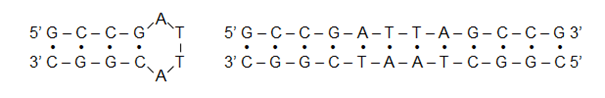
\includegraphics[width=1\columnwidth]{dna_hairpins/structure}
	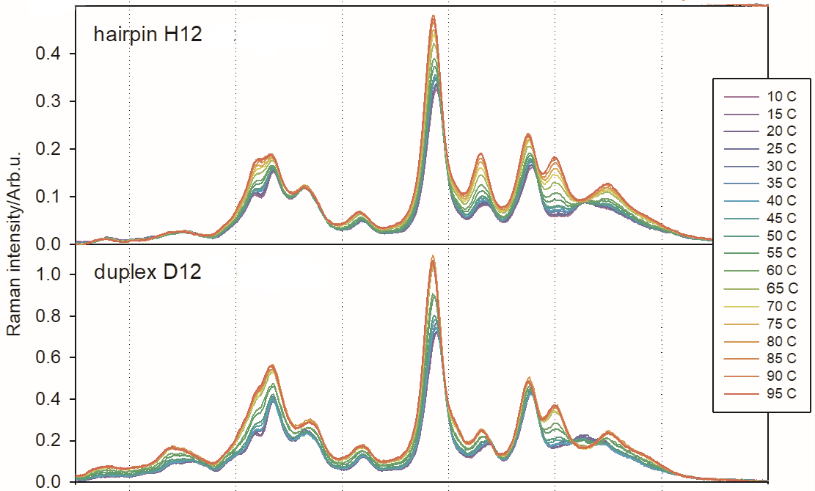
\includegraphics[width=.9\columnwidth]{dna_hairpins/melting_spectra}
\end{center}
\end{frame}

\begin{frame}{Analýza vlivu teploty na strukturu DNA}
\begin{center}
	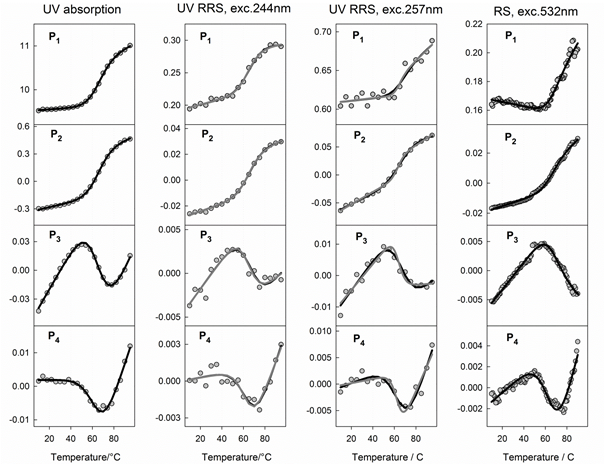
\includegraphics[width=.9\columnwidth]{dna_hairpins/pca_hairpin}
\end{center}
\end{frame}

\begin{frame}{Analýza vlivu teploty na strukturu DNA}
\begin{center}
	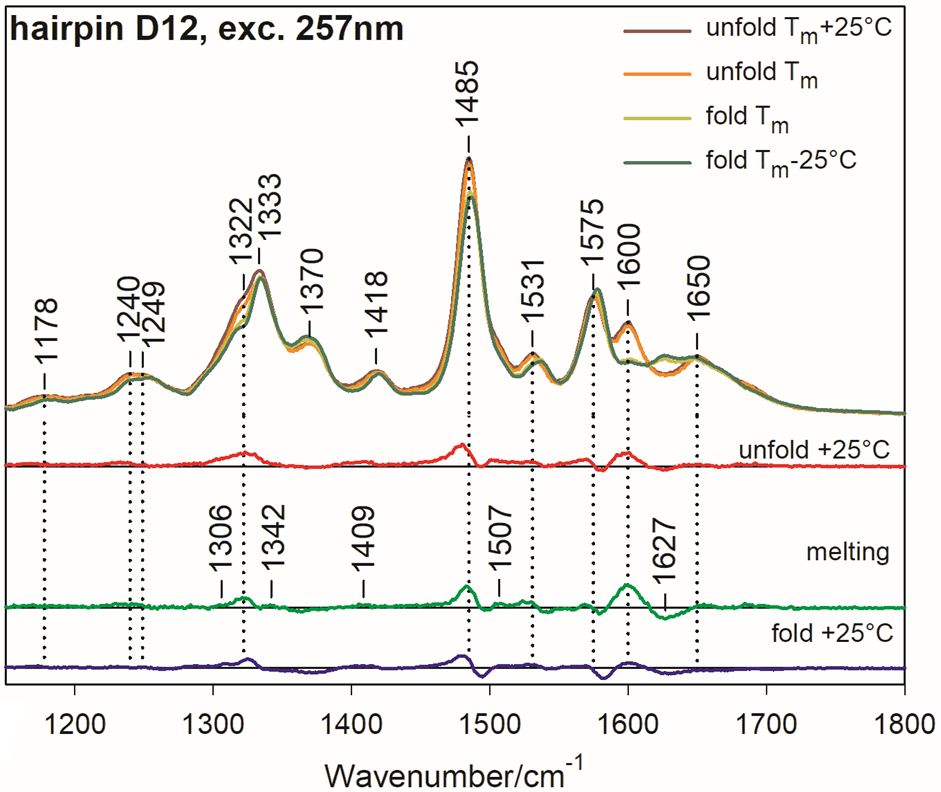
\includegraphics[width=.9\columnwidth]{dna_hairpins/forms_spectra}
\end{center}
\end{frame}

\begin{frame}{Analýza vlivu teploty na strukturu DNA}
\begin{figure}
	\centering
	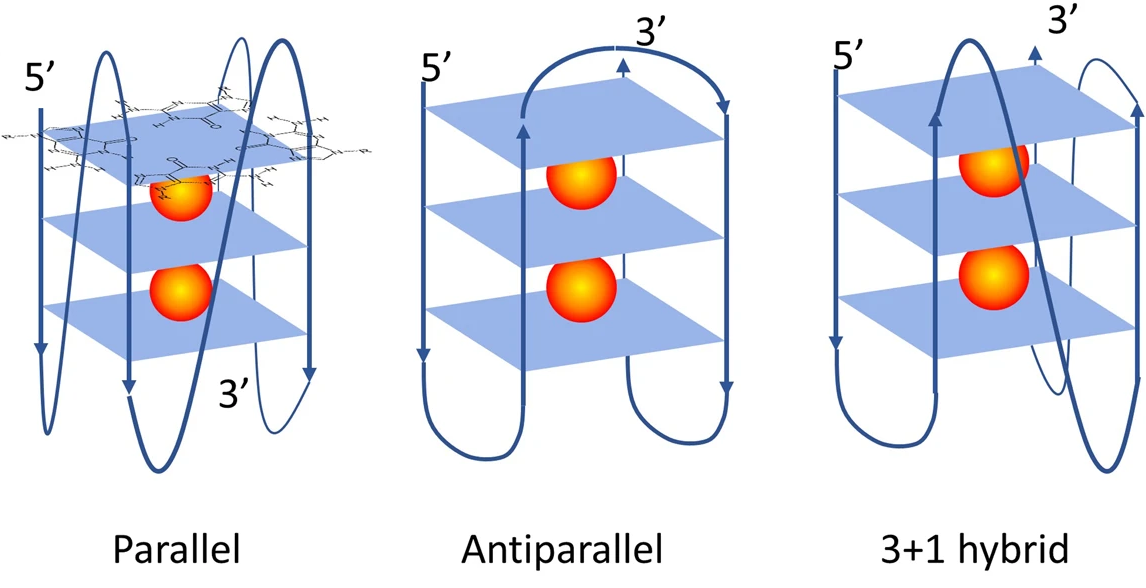
\includegraphics[width=1\columnwidth]{tel22/quadruplex_forms}\\
	\caption*{
		Benabou S. et al., 2019.
		\emph{Sci. Rep.}
		\textbf{9}(15807), 1.
	}
\end{figure}
\end{frame}

\begin{frame}{Studium přechodu mezi paralelním a antiparalelním\\ kvadruplexem}
\begin{center}
	\resizebox{1\columnwidth}{!}{\input{tel22/tel22_spectra}}
\end{center}
\end{frame}


\refstepcounter{section}% Increase section counter
\sectionmark{Shrnutí}% Add section mark (header)
\addcontentsline{toc}{section}{\protect\numberline{}\thesection. Shrnutí\par}%

\begin{frame}{Shrnutí}
\begin{itemize}
	\item Byl postaven UV Ramanův spektrometr
	\begin{itemize}
		\item Byla vyvinuta metoda kalibrace vlnočtové škály
		\item Možnost měření v pravoúhlé geometrii i geometrii zpětného rozptylu
		\item Zkonstruována rotační cela
		\item Zkonstruován držák na kyvety umožňující teplotně závislá měření
		\item Optimalizovány podmínky měření
	\end{itemize}
	\item Vytvořena interpretační tabulka rezonančních Ramanových spekter
		nukleových kyselin
	\item Nalezená metodologie byla aplikována na několik strukturních studií
		nukleových kyselin
\end{itemize}
\end{frame}


\end{document}